\section{Hintergrund}\label{kapitel1}

Beschreibung warum die subsections Teil der Arbeit sind. 

%- Beschreibung Arnika (Zusammenfassung)
%- Botanische Beschreibung 
%- Medizinische Nutzung
%   - Umstrittene Nutzung innerer Anwendung bei Herz- Kreislaufbeschwerden (Goethe Zitat)
% - Naturschutzstatus
% - Anbau und Schwierigkeiten -> weitere Notwendigkeit der nachhaltigen Wildsammlungen v.A. in Rumänien
\subsection{\textit{Arnica montana}}

\begin{quotation}
„Wenn man nur eine einzige Pflanze in der Hausapotheke haben könnte, so würde ich zu Arnika raten.“ \citep[S. 186]{Sommer2011}
\end{quotation}

\textit{Arnica montana}, auch „Bergwohlverleih“ genannt, ist eine Arzneipflanze, die seit Jahrhunderten wegen ihrer tiefen Heilwirkung bekannt ist und verwendet wird. Die vermutlich erste Erwähnung fand Arnika bei Hildegard \citet{Bingen2007}, die sie in ihrem Buch von den Pflanzen von 1151–1158 „Woluis gelegena“ nennt. Sie beschreibt Arnika als Liebesmittel zur äußeren Anwendung. Arnika sei „sehr warm und hat eine giftige Wärme in sich“. Die erste Erwähnung als Arzneipflanze findet sich 1588 im Kräuterhandbuch von Tabernaemontanus, eigentlich Jacob Theodor aus Bergzabern. In der breiten Bevölkerung wird Arnika ab dem 18. Jahrhundert bei Krankheiten und Beschwerden eingesetzt. Deshalb tauchte sie auch im Herbarium Backwellium von Elizabeth \citet{Blackwell1757} und dem Medizinal von Franz Eugen \citet{Kohler1887} auf (Siehe Abbildung~\ref{fig:Zeichnung}, S.\pageref{fig:Zeichnung}).

\begin{figure}[htb]
    \subfigure[]{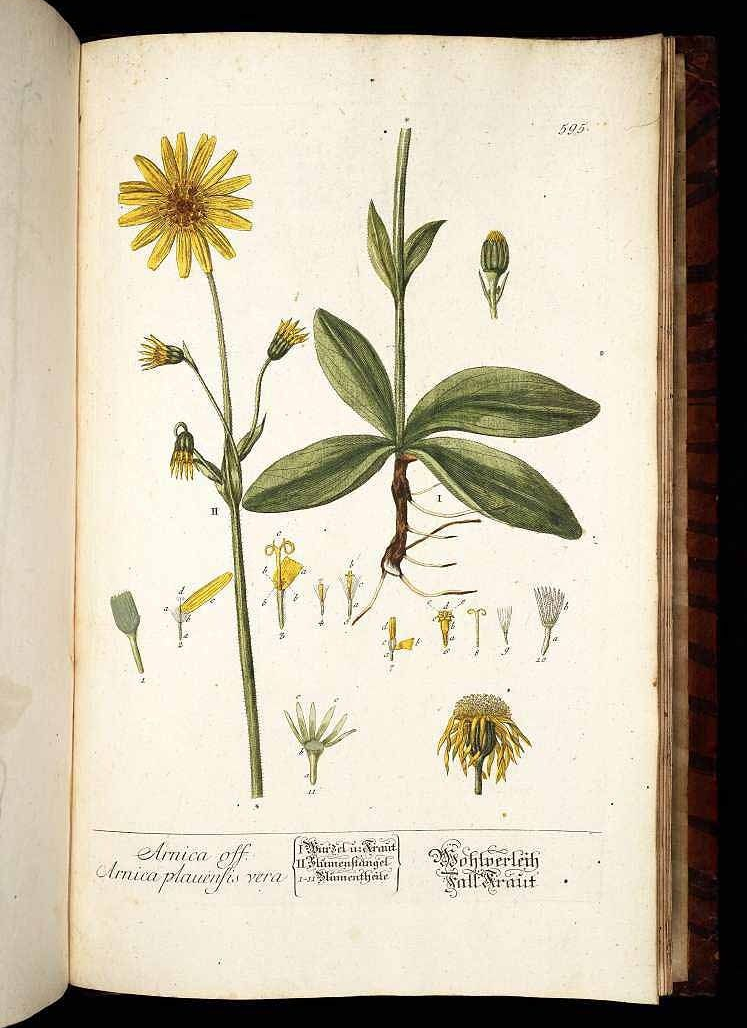
\includegraphics[width=0.49\textwidth]{abb/herbarium-blackwell}}
    \subfigure[]{\includegraphics[width=0.49\textwidth]{abb/Koehler-medizinal-pflanzen}}
\caption{\textit{Arnica montana} aus \citet{Blackwell1757} (a) und \citet{Kohler1887} (b)}
  \label{fig:Zeichnung}
\end{figure}

Aufgrund ihrer fiebersenkenden Wirkung galt sie lange als das „Chinin der armen Leute“. Sebastian Kneipp hat angeblich täglich mit Arnikatee gegurgelt. „Arnika ist nicht mit Gold zu bezahlen“, soll er gesagt haben. Auch Johann Wolfgang nutzte Arnika: Er erholte sich 1823, 10 Jahre vor seinem Tod, vermutlich von einem Herzinfakt durch eine Tasse Arnikatee \citep[vgl.][S.56]{Franke2012}.

Die \textit{Arnica montana} zählt zu den Korbblütern (botanisch Asteraceae oder Compositae) und ist eine mehrjährige Staudenpflanze, die meist eine maximale Höhe von 30 bis 60 cm erreicht. Die behaarten Blätter haben eine elliptische Form und sind in am Boden anliegenden Rosetten angeordnet. Zusätzlich hat die \textit{Arnica montana} ein bis drei gegenständige Stängelblätter \citep[vgl.][]{Wyk2015, FNR2013}. Eine Pflanze besitz ein bis drei 5-8 cm breite Blütenköpfe mit gelb-orangen dreigezähnten Zungen- oder Röhrenblüten. Die Blütezeit ist von Juni bis August. \textit{Arnica montana} steht auf Magerrasen, Wiesen, trockenen Mooren und Heiden, sowie in lichten Nadelwäldern. Sie ist als Wildpflanze bis in die alpine Stufe weiter Teile Europas zu finden \citep[vgl.][]{Schoenfelder2011, FNR2013}.

Es gibt zwei Unterarten (subsp.) bei der \textit{Arnica montana}: \textit{montana} und \textit{atlantica}. Die \textit{Arnica montana ssp. montana} ist die sogenannte alpine Arnika, die vor allem in Höhenlagen Mittel und Osteuropas zu finden ist. Die \textit{Arnica montana ssp. atlantica}, wird auch spanische Arnika genannt und ist nur in den französischen und spanischen Pyrenäen und im Norden Spaniens und Portugals zu finden. Die Blüten der spanischen Arnika sind etwas kleiner und heller als bei der alpinen Arnika, sie ähnelt damit der nordamerikanischen \textit{Arnica chamissonis} (Siehe Abbildung~\ref{fig:Unterarten}, S.\pageref{fig:Unterarten}) \citep[vgl.][S. 61]{Franke2012}.

\begin{figure}[htb]
 \centering
 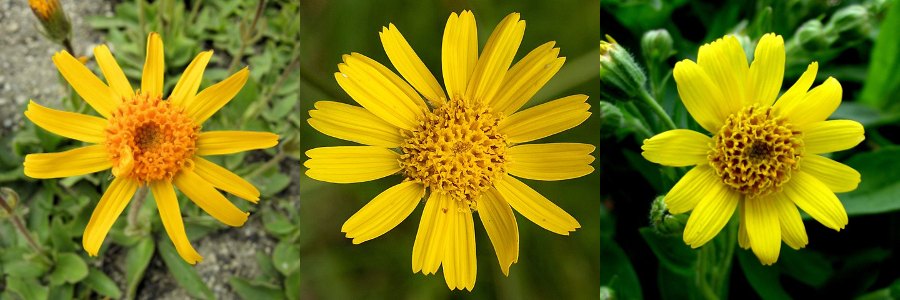
\includegraphics[width=\textwidth,angle=0]{abb/Arnika/arnica-900x300}
 \caption{v.l.n.r.: alpine Arnika \citep{Moro2019}, spanische Arnika \citep{Pereira2019} und nordamerikanische Wiesen-Arnika \citep{Rowlin2019}}
\label{fig:Unterarten}
\end{figure}

\subsubsection{Medizinische Wirkung}

Die ganze Arnika-Pflanze enthält Wirkstoff. Früher wurden vor allem Wurzeln zur medizinischen Anwendung genutzt, heute meist nur die Blüten, auch Arnicae Flos oder Flores Arnica (montanae) genannt \citep[vgl.][S. 144 f.]{Roth2012}. Die Hauptwirkstoffe der Blüten (0,1-0,5\%) sind die Sesquinterpenlactone (SL) Helenalin und Dihydrohelenalin sowie deren Ester. SL können kovalente Bindungen mit Proteinen eingehen und so deren Aktivität verändert \citep[vgl.][S. 62]{Wyk2015}. Durch Helenalin kann die Vermehrung von Mikroorganismen gehemmt werden, was Entzündungen entgegen wirkt \citep[vgl.][S. 32 f.]{FNR2013}. \citet[S. 73 f.]{Schoenfelder2011} schreibt: „Die Helenalinester sind gleichzeitig für die Nebenwirkungen verantwortlich, vor allem die relativ häufig auftretenden allergisch bedingten Hautreaktionen nach äußerer Anwendung“. Andere Inhaltsstoffe von Arnika sind Flavone (gelbe Pflanzenfarbstoffe) und Flavonoide. Auf Flavonoide lässt sich ebenfalls die entzündungshemmende Eigenschaft von Arnika zurück verfolgen. Außerdem enthält \textit{Arnica montana} verschiedene ätherische Öle, Trierpenalkohole, Phenolcarbonsäuren und Polysaccharide \citep[vgl.][]{Wyk2015, Schoenfelder2011}. Insgesamt gibt es bei dem Inhaltsstoffen und deren Mengen erhebliche Schwankungen je nach Standort \citep[vgl.][S. 144 f.]{Roth2012}.

% -Wirkung und äußere Anwendung
Arnika wirkt entzündungshemmend, schmerzstillend, antiseptische, durchblutungssteigernd und wundheilend. Traditionell wird Arnika als alkoholische Tinktur, auch „Arnika-Schnaps” genannt, verdünnt zum Einreiben oder für Umschläge verwendet. Im Handel gibt es heute daneben vor allem Salben und Cremes sowie homöopathische Zubereitungen \citep[vgl.][S. 32 f.; S. 399]{FNR2013, Prentner2017}. Angewendet wird Arnika äußerlich zur Behandlung von stumpfen Verletzungen, Hämatomen, Quetschungen, Ödemen, Verrenkungen, Verstauchungen, Muskelschmerzen, Gelenkschmerzen, Venenbeschwerden oder rheumatischen Beschwerden. Auch bei Schleimhautentzündungen in Mund und Rachen, so wie Insektensticken oder Sonnenbrand kann Arnika angewendet werden \citep[vgl.][]{Roth2012, Prentner2017, Wyk2015, FNR2013, Schoenfelder2011}.

%Studie zur Homöopatischen Wirksamkeit im vergleich zu diclofenac (orale Einnahme) ???

%Nebenwirkungen und Allergiepotential
Bei längerer Anwendung an geschädigter Haut oder bei zu hoher Konzentration kann es Nebenwirkungen in Form von Ekzemen, ödematöser Dermatitis oder eiterhaltiger Bläschenbildung, bis hinzu Nekrotisierung, kommen \citep[vgl.][S. 144 f.]{Roth2012}. Eine Einnahme kann beim Mensch zur Reizung des Magen-Darm-Traktes, Kopfschmerz, Erschwerung der Atmung, starkem Herzklopfen und Schwindelgefühl führen \citep[vgl.][S. 144 f., S.178]{Roth2012, Schoenfelder2015}. Beim Tier beschreiben \citet{Roth2012} ähnliche Symptome: „Wirkungen auf Nerven- und Gefäßsystem, Beschleunigung der Atmung, Vermehrung der Schweiß- und Harnabsonderung“. Zusätzlich zu den Nebenwirkungen kann Arnika kontaktallergische Reaktionen auslösen, diese sind auf das Helenalin zurückzuführen. Bei einer bekannten Überempfindlichkeit gegen Korbblüter sollte Arnika nicht angewendet werden \citep[vgl.]{Schoenfelder2015, FNR2013, Wyk2015}. 
Die spanische Arnika hat ein wesentlich geringeres Allergiepotenzial, da sie statt Helenalin Dihydrohelenalin enthält. Einigen Studien zufolge ist das Allergie und Nebenwirkungsrisiko insgesamt bei Arnika gering, wenn eine korrekte Anwendung und niedrige Dosierung erfolgt. Eine Untersuchung der Allergie-Forschungsgruppe der Hautklinik Freiburg hat sogar ergeben, dass bei der äußeren Anwendung von Arnika nicht nur keine kontaktallergene Reaktionen festgestellt werden konnten, sondern die entzündungshemmende Wirkung der Arnika einer Allergie und möglichen Schwellungen entgegenwirkt \citep[vgl.][S. 448]{Buehring2014}

% innere Anwendung
Die innere Anwendung oder Einnahme von Arnika ist sehr umstritten und wird heute meist abgelehnt. \citet[S. 144 f.]{Roth2012} und \citet[S. 62]{Wyk2015} warnen aufgrund von toxischen Nebenwirkungen vor der Einnahme, da diese zu Fehlgeburt oder sogar zum Tod führen kann. \citet[S. 73 f.]{Schoenfelder2011} und \citet[S. 32. f]{FNR2013} raten ebenfalls von einer innerlichen Anwendung ab, außer im Bereich der Homöopathie. Bei \citet[S. 40 f.]{Prentner2017} hingegen wird \textit{Arnica montana} unter den „Heilpflanzen bei koronaren Herzerkrankungen“ aufgeführt. Sie beschreibt sie als „akutes Herzmittel bei akuten Schwächezuständen des Herzens und bei Angina pectoris“ zusätzlich schreibt \citet[S. 40 f]{Prentner2017} Arnika „eine stärkende Wirkung auf Gefäßnerven, Herznerven und Blutgefäße“ und insbesondere „Verbesserung der Durchblutung der Herzkranzgefäße“ zu. Aber auch \citet[S. 40 f.]{Prentner2017} warnt vor einer längeren Anwendungsdauer oder zu hoher Dosierung mit den bekannten Nebenwirkungen.

\subsubsection{Naturschutzstatus}

Seit dem 1. Januar 1987	zählt \textit{Arnica montana} in Deutschland zu den besonders geschützte Arten nach § 1 Satz 1 der Verordnung zum Schutz wild lebender Tier- und Pflanzenarten (Bundesartenschutzverordnung - BArtSchV). Laut dem Bundesnaturschutzgesetz (BNatSchG) ist es verboten „wild lebende Pflanzen der besonders geschützten Arten oder ihre Entwicklungsformen aus der Natur zu entnehmen, sie oder ihre Standorte zu beschädigen oder zu zerstören” (§ 44 Abs. 1 Satz 4, BNatSchG). Außerdem ist der Besitz und die kommerzielle Nutzung nach § 44 Abs. 2 Satz 1-2 BNatSchG untersagt.

In der Roten Liste gefährdeter Tiere, Pflanzen und Pilze Deutschlands (RL), herausgegeben durch das \citet[S. 36]{RL2018} wird \textit{Arnica montana} als „RL-Kategorie 3: Gefährdet” eingestuft. Die RL wird nach einer Sammlung von wissenschaftlichen Fachgutachten erstellt und soll das aktuelle Ausmaß der Gefährdung dieser Arten in Deutschland dokumentieren und bewerten. Die RL wird in der BRD und DDR seit den 1970er Jahren erstellt und sollen etwa alle zehn Jahre aktualisiert werden. Sie dienen  auch als Argumentationshilfe und Grundlage für Maßnahmen des Naturschutzes auf legislativer Ebene \citep[vgl.][]{RL2009}. %% kürzen? RL nur in einem Satz erklären

\textit{Arnica montana} fällt im hohen Maße in die Verantwortlichkeit Deutschlands laut RL. Die aktuelle Bestandssituation wird als „mäßig häufig“ bezeichnet. Dies entspricht einer Rasterfrequenz von 10-30 \% (bei n = 3000) oder 301-1000 TK25-Rasterfelder, die im Bezug zur Gesamtzahl der Topographischen Karten im Maßstab 1 : 25.000 (TK 25) mit Artnachweisen gesetzt wurden. Laut RL ist bei \textit{Arnica montana} ein starker Rückgang im langfristigen Bestandestrend im den letzten 100-150 Jahren zu beobachten. Der kurzfristige Bestandestrend der letzten 25 Jahre beschreibt nur eine „mäßge Abnahme oder [ist] im Außmaß unbekannt” \citep[S. 36]{RL2018}. Andere Risikofaktoren, die eine Verschlechterung der Bestandesentwicklung in den kommenden zehn Jahren erwarten, sind nicht feststellbar. Im Vergleich zur RL von 1998 gibt es keine Kategorieänderung der Gefährdeeinstufung von \textit{Arnica montana} \citep[vgl.][S. 36]{RL2018}. Weiter wird in der RL vom \citet[S. 148]{RL2018} angemerkt: „Die Bestände außerhalb des Berglandes sind stärker gefährdet“. %%Kürzen?? Und nur Gefährdestatus und Entwicklung beschreiben?

%% mehr aktiv beschreiben: Es haben Schutzmaßnahmen wirkung gezeigt, zB. Pflegemaßnahmen in bei Magerrasen (siehe Quelle) oder Bundesprogramm Biologische Vielfalt Siehe Quelle 2. Obwohl in der Schweiz gesetzlich \textit{Arnica montana} XY Status hat, ist in den Rote Liste Schweiz (2002)(pdf) der Gefährdestatus mittlerweile XY. evtl. anderer Status RL Schweiz im Vergleich zu Deutschland ??

Europaweit variiert der Naturschutzstatus der \textit{Arnica montana} und somit auch die Naturschutzmaßnahmen in den jeweiligen Ländern. Nach der EU Fauna-Flora-Habitat-Richtlinie (FFH-Richtlinie) von 1997 ist Arnika eine Art vom gemeinschaftlichem Interesse, für die vorangig Schutzgebiete ausgewiesen werden sollen. Zusätzlich wird nach EU Verordnung 2017/160 der Kommission vom 20. Januar 2017 die Einfuhr von lebenden, sowie getrockneten oder frischen Pflanzen oder Pflanzenteilen der \textit{Arnica montana} überwacht. Nach Verordnung Nr. 338/97 des Rates vom 9. Dezember 1996 „über den Schutz von Exemplaren wildlebender Tier- und Pflanzenarten durch Überwachung des Handels“ sind die Vollzugsbehörden der Mitgliedstaaten zu jährlichen Berichten über den Umfang der Gemeinschaftseinfuhren verpflichtet. %(kürzen? nur ein Satz, seit XY wird der Handel überwacht

In Belgien, Luxemburg, Kroatien und Bosnien und Herzegowina gilt \textit{Arnica montana} als „vom Aussterben bedroht“. „Stark gefährdet“ ist der Naturschutzstatus in Holland und Weißrussland, „gefährdet“ in Deutschland, Litauen, Lettland, Estland, Rumänien und Kaliningrad. In Norwegen und Dänemark ist \textit{Arnica montana} „beinahe gefährdet“.
In Teilen der Schweiz, Regionen von Frankreich (Zentralmassiv und Bourgogne) und Ungarn ist \textit{Arnica montana} streng geschützt. Im Alpenraum ist das Sammeln von Blüten generell untersagt. In weiteren sieben Regionen Frankreichs und in Rumänien ist eine Sammellizenz erforderlich. In Spanien ist die Sammlung bislang völlig unkontrolliert. Darüber hinaus werden dort und in Portugal durch EU-Maßnahmen die Trockenlegung von Feuchtflächen gefördert, was den Bereich der Arnika weiter einschränkt \citep[vgl.][]{Franke2012}.

\subsubsection{Gewinnung}  

%Bodenansprüche der \textit{Arnica montana}
Die \textit{Arnica montana} ist sehr empfindlich gegenüber bestimmten Bodentypen und Düngung. Sie gedeiht am besten auf nährstoffarmen, gut durchlüftetem Boden mit einer guten Wasserzu- und abfuhr. Die Pflanzen sind gegen Kälte widerstandsfähig und vertragen auch starke Sonnenstrahlung. Ebenfalls heftige Niederschläge kann die \textit{Arnica montana} aushalten, wenn keine Staunässe im Boden bleibt. Der ideale pH-Wert des Bodens sollte zwischen 5 und 6,2 liegen und damit leicht sauer sein. \textit{Arnica montana} benötigt viel Kieselsäure, die Stängel und Blätter stärkt und Einfluss auf Ungeziefer hat. Der CaCO3-Gehalt im Boden darf 1,5\% nicht überschreiten, da es sonst zu Verfärbungen (Chlorosen), Wachstumstörungen und Pflanzenausfall kommen kann \citep[vgl.][]{Franke2012, FNR2013, Heeger1956}.


Wegen dieser schwierigen Bedingungen wurde Arnika zur Arzneimittelherstellung viele Jahre größtenteils aus Wildpflückung der \textit{Arnica montana} bezogen, was bereits seit dem 18. und 19. Jahrhundert zum Rückgang der Art beitrug. In den letzten Jahrzehnten kamen zwei weitere Belastungsfaktoren hinzu. Vermehrte landwirtschaftliche Nutzung von mageren Wiesen und die damit einhergehende Düngung und die Verbrachung von zuvor genutzen Flächen sorgen dafür, dass diese als Standort für Arnika nicht länger geeignet sind \citep[vgl.][]{Franke2012}.
Aufgrund des Artenschutzes der \textit{Arnica montana}, war zeitweise die \textit{Arnica chamissonis} bis 2002 als Stammpflanze für pharmazeutische Arnika-Produkte im Handel zugelassen. Die ursprünglich nordamerikanische \textit{Arnica chamissonis} (Siehe Abbildung~\ref{fig:Unterarten}, S.~\pageref{fig:Unterarten}) hat ähnliche Inhaltstoffe wie die europäische \textit{Arnica montana}, sie ist aber wesentlich leichter zu kultivieren. Inzwischen ist es aber Pflanzenzüchtern gelungen, eine für den Feldanbau geeignete Sorte von \textit{Arnica montana} zu entwickeln. Seit 1998 gibt es für die Sorte "Arbo" der \textit{Arnica montana} montana Sortenschutz \citep[vgl.][S. 178]{Schoenfelder2015}.


Naturkosmetik und -Arzneimittelhersteller in Europa haben verschiedene Wege gewählt, um im Einklang mit dem Naturschutz Arnika für ihre Produkte zu gewinnen. Der französische Naturkosmetikhersteller Yves Rocher verwendet seit 1983 nur noch die \textit{Arnica chamissonis}. Bis heute decken sie mit einer speziellen Züchtung ihren Bedarf durch Feldanbau der \textit{Arnica chamissonis} in der Bretagne im Nordwesten Frankreichs \citep[vgl.][]{Rocher2019}. Kneipp, ein Hersteller von Naturheilkundeprodukten aus Bayern, wählt die spanische Arnika für seine Produkte. Neben dem Bezug aus Wildsammlungen in Nordspanien, investiert Kneipp in neue Züchtungen, die einen Anbau möglich machen sollte. Mit der firmeneigener Sorte „Arvita“ versuchte Kneipp ab 2011 auch den Anbau in Deutschland durchzuführen. Dies erwies sich aber als nicht wirtschaftlich, da nur 25\% der Pflanzen dem strengen Winter und langen Trockenperioden Mitteleuropas stand hielten. Seit 2013 fördert Kneipp ein Pilotprojekt zum Anbau in Nordspanien und weitet dort die nachhaltige und kontrollierte Wildsammlung weiter aus \citep[vgl.][]{Kneipp2019, Markenverband2019}.

\begin{figure}[htb]
 \centering
 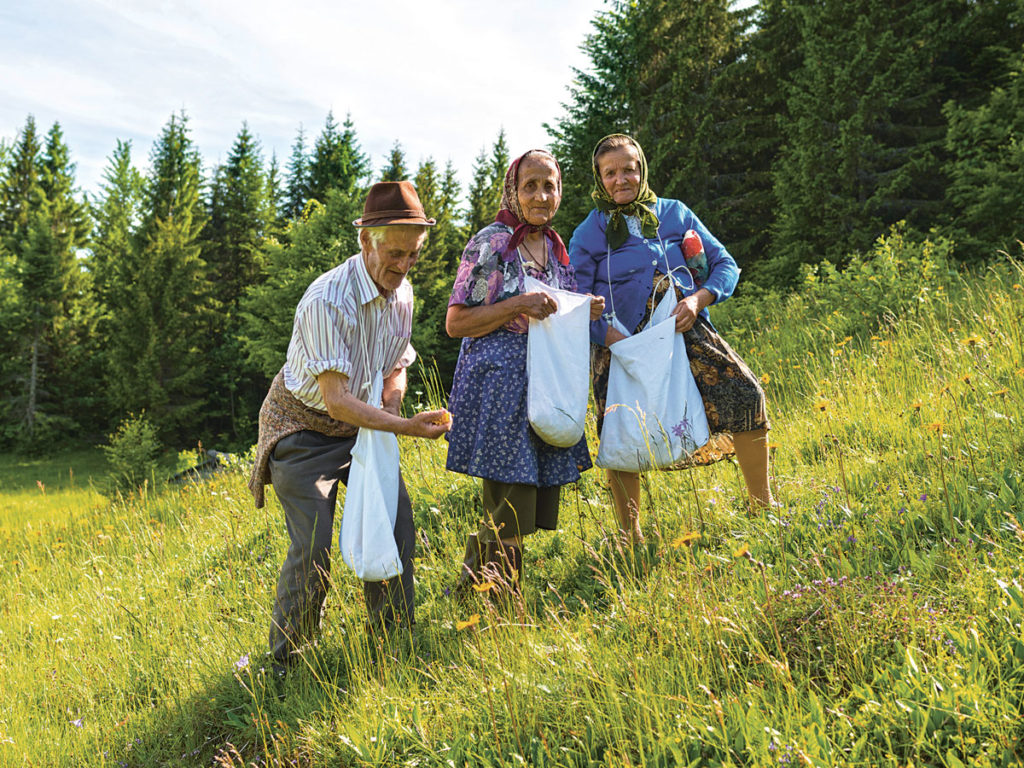
\includegraphics[width=0.8\textwidth,angle=0]{abb/Arnika/Arnikapfluecker-1024x768}
 \caption{ArnikapflückerInnen in den Karparten \citep{Mestrovic2019}}
\label{fig:pfluecker}
\end{figure}

Der Arznei- und Naturkosmetikhersteller Weleda aus Schwäbisch Gmünd setzt, nach ebenfalls vergeblichen Versuchen \textit{Arnica montana} in Deutschland anzubauen, auf nachhaltige Wildsammlungen im Apuseni-Gebirge in Rumänien (Siehe Abbildung~\ref{fig:pfluecker}, S.\pageref{fig:pfluecker}). Das seit 2010 bestehenden rumänischen Unternehmen Bioflora Apuseni führt nachhaltige Wildpflückungen durch und setzt sich dafür ein, dass das Grünland nur durch extensive Viehwirtschaft und ohne jegliche zusätzliche Düngergaben genutzt wird. Die von Hand gepflückten Blüten werden vor Ort in einer von Weleda finanzierten Trocknungsanlage getrocknet. Weleda möchte die Wildsammlungen in weiteren Teilen der Karparten ausdehnen, um auch dort durch Bewirtschaftung die Biodiversität zu erhalten \citep[vgl.][]{Weleda2019}. 
